Graphs are fundamental data structures in many applications, such as social networks, recommendation systems, and biological networks. In recent years, a number of high performance graph processing frameworks have emerged. State-of-the-art frameworks include Gunrock \cite{wang2016gunrock}, Hornet \cite{busato2018hornet}, Ligra \cite{shun2013ligra}, and Galois \cite{nguyen2013lightweight}. Their emphasis lies in accelerating graph analytics tasks by providing high-performance kernels tailored to diverse datasets.

However, fast graph loading is crucial for minimizing the time it takes to start processing and analyzing the graph data. Unfortunately, loading graph data is a significant bottleneck in such frameworks \cite{gabert2021pigo}, where the cost of loading data can dominate the overall processing time - especially as computational capabilities continue to improve. This motivates us to work on efficient IO techniques. These not only improve response time, but also help lower system / cloud usage charges.

\ignore{Recent graph computation approaches have demonstrated that a single PC can perform efficiently on billion-scale graphs. While these approaches achieve scalability by optimizing I/O operations, they do not fully exploit the capabilities of modern hard drives and processors \cite{gualdron2016m}.}

\ignore{Many implementations persist with sequential I/O, and the article challenges the prevalent notion that parallel I/O is unattainable without dedicated systems. By exploring opportunities for parallelism through hardware RAID controllers, Non-Volatile Memory (NVM), and file system caches, the article introduces a pragmatic perspective on addressing I/O challenges. Gabert et al. present PIGO, a lightweight C++11 header-only library, as a solution that, without imposing the complexities of existing graph systems, significantly enhances end-to-end performance and productivity for researchers and developers working on shared-memory multi-core servers. Experimental results underscore PIGO's potential to redefine the landscape of optimized graph loading, complementing the strengths of popular graph processing frameworks \cite{gabert2021pigo}.}




% - Why fast graph loading is important?
% - Extremely high cost of loading compared to computation.
% - An issue with even popular graph processing frameworks.
% - Modern IO is fast (compared to CPU performance).
% - Storage capacities increasing, bandwidth is high, CPUs as not as fast as they used to be.
% - Common graph file formats (COO, MTX).
% - Common memory storage formats (Edgelist, CSR).
% - Work presented in this paper.




%% - Use --- for a dash.
%% - Use ``camera-ready'' for quotes.
%% - Use {\itshape very} or \textit{very} for italicized text.
%% - Use \verb|acmart| or {\verb|acmart|} for mono-spaced text.
%% - Use \url{https://capitalizemytitle.com/} for URLs.
%% - Use {\bfseries Do not modify this document.} for important boldface details.
%% - Use \ref{fig:name} for referencing.

%% For a block of pre-formatted text: 
% \begin{verbatim}
%   \renewcommand{\shortauthors}{McCartney, et al.}
% \end{verbatim}

%% For a list of items:
% \begin{itemize}
% \item the ``ACM Reference Format'' text on the first page.
% \item the ``rights management'' text on the first page.
% \item the conference information in the page header(s).
% \end{itemize}

%% For a table:
% \begin{table}
%   \caption{Frequency of Special Characters}
%   \label{tab:freq}
%   \begin{tabular}{ccl}
%     \toprule
%     Non-English or Math&Frequency&Comments\\
%     \midrule
%     \O & 1 in 1,000& For Swedish names\\
%     $\pi$ & 1 in 5& Common in math\\
%     \$ & 4 in 5 & Used in business\\
%     $\Psi^2_1$ & 1 in 40,000& Unexplained usage\\
%   \bottomrule
% \end{tabular}
% \end{table}

%% For a full-width table:
% \begin{table*}
%   \caption{Some Typical Commands}
%   \label{tab:commands}
%   \begin{tabular}{ccl}
%     \toprule
%     Command &A Number & Comments\\
%     \midrule
%     \texttt{{\char'134}author} & 100& Author \\
%     \texttt{{\char'134}table}& 300 & For tables\\
%     \texttt{{\char'134}table*}& 400& For wider tables\\
%     \bottomrule
%   \end{tabular}
% \end{table*}


%% For inline math:
% \begin{math}
%   \lim_{n\rightarrow \infty}x=0
% \end{math},

%% For a numbered equation:
% \begin{equation}
%   \lim_{n\rightarrow \infty}x=0
% \end{equation}

%% For an unnumbered equation:
% \begin{displaymath}
%   \sum_{i=0}^{\infty} x + 1
% \end{displaymath}

%% For a figure:
% \begin{figure}[h]
%   \centering
%   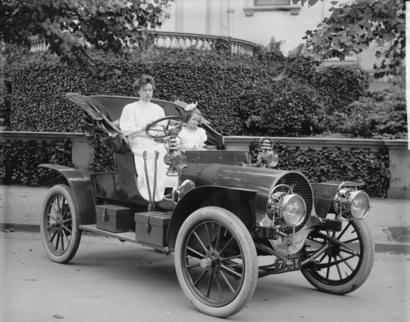
\includegraphics[width=\linewidth]{inc/sample-franklin}
%   \caption{1907 Franklin Model D roadster. Photograph by Harris \&
%     Ewing, Inc. [Public domain], via Wikimedia
%     Commons. (\url{https://goo.gl/VLCRBB}).}
%   \Description{A woman and a girl in white dresses sit in an open car.}
% \end{figure}

%% For a teaser figure.
% \begin{teaserfigure}
%   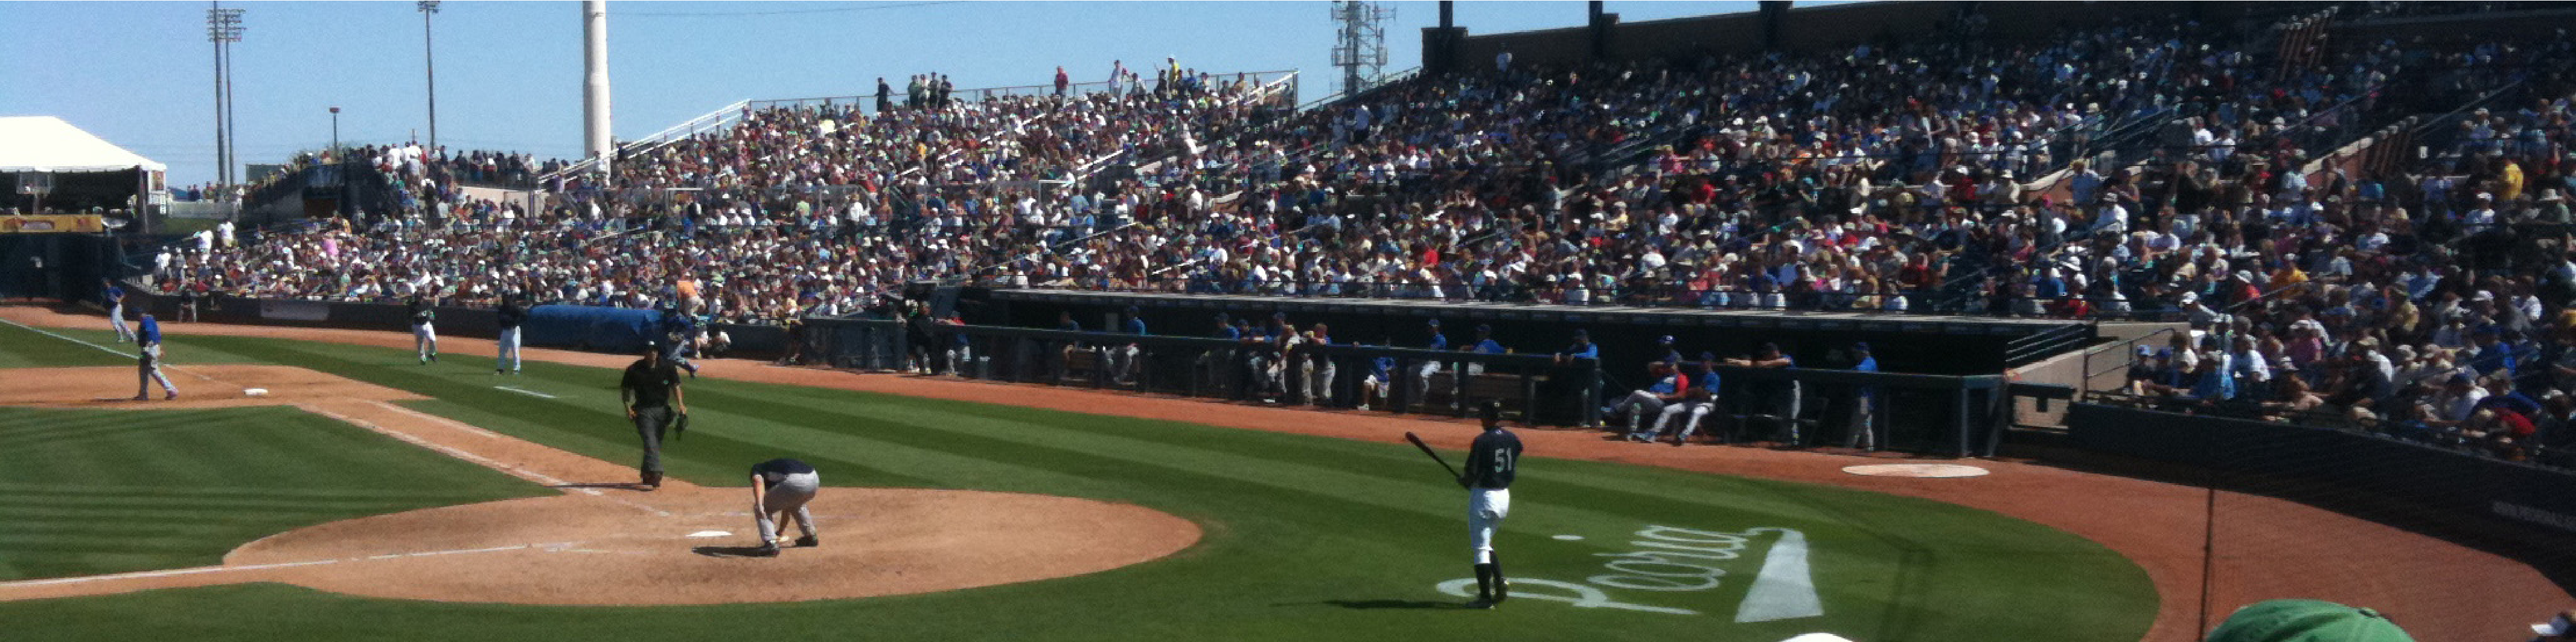
\includegraphics[width=\textwidth]{sampleteaser}
%   \caption{figure caption}
%   \Description{figure description}
% \end{teaserfigure}
